% EF5342 Week 7 — Foreign Exchange Markets
% Beamer conversion from week7_FXmarkets.pptx (61 source slides -> 41 frames).
% Compile: pdflatex week7_FXmarkets.tex
% Each frame carries a [src: ...] comment mapping back to source slides.
\documentclass[aspectratio=169]{beamer}
\usepackage{../ef5342}

\title{EF5342 Financial Systems, Markets and Instruments}
\subtitle{Week 7 --- Foreign Exchange Markets}
\author{Prof.\ Weikai Li}
\institute{City University of Hong Kong}
\date{Semester B 2026--2027}

\begin{document}

% ============ OVERVIEW ============

% [src: 1]
\begin{frame}
\titlepage
% Title-page background image (slide01_img0.jpg) dropped — decorative.
\end{frame}

% [src: 2, 3]
\begin{frame}{The Foreign Exchange Market}
\textbf{Outline:} overview of FX markets; quotes and trades; hedging FX risk; how exchange rates move; the carry trade and other currency strategies.
\vspace{0.4em}
The FX market's three functions:
\begin{description}
  \item[Currency conversion] Facilitates conversion of one country's currency into another --- global firms move in and out of foreign currency as needed
  \item[Setting exchange rates] The ratio of one currency to another; these rates determine costs and returns to global businesses
  \item[Hedging contracts] Allow firms to offset foreign-currency exposure and manage FX risk --- so they can concentrate on their core business
\end{description}
\end{frame}

% [src: 4]
\begin{frame}{Spot and Forward Transactions}
FX markets are where one currency is exchanged for another, today or at a set future date:
\begin{description}
  \item[Spot] Immediate exchange at current rates --- $\sim$27\% of global FX turnover
  \item[Forward] Exchange at a specified rate on a specific future date --- 19\% of turnover
  \item[FX swaps] A spot leg plus an opposite forward leg, usually identical in notional --- 42\% of turnover
\end{description}
\begin{columns}
\begin{column}{0.44\textwidth}
\begin{figure}
\centering
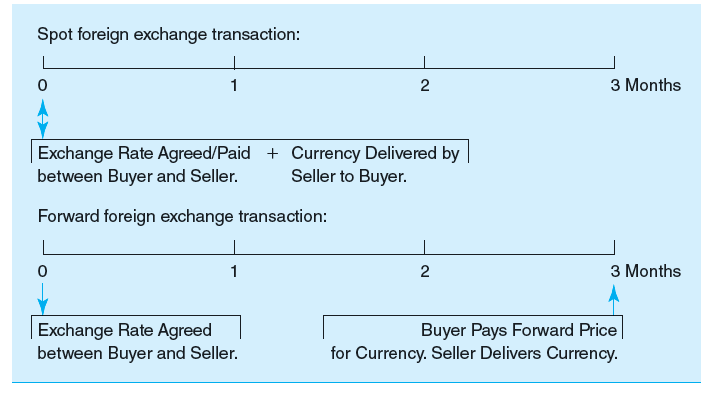
\includegraphics[width=\linewidth,keepaspectratio]{figures/slide04_img0.png}
\end{figure}
\end{column}
\end{columns}
\end{frame}

% [src: 5, 6]
\begin{frame}{Market Participants}
\textbf{Four tiers} by information advantage, motivation, and market access:
\begin{table}
\centering
\footnotesize
\begin{tabular}{lp{0.42\textwidth}p{0.36\textwidth}}
\toprule
\textbf{Tier} & \textbf{Participants} & \textbf{Primary motivation} \\
\midrule
1 (Core) & Major dealer banks (JPMorgan, UBS, Deutsche, Citi, Barclays) & Market-making, proprietary trading \\
2 (Interbank) & Regional and smaller banks & Customer service, hedging, arbitrage \\
3 (Buy-side) & Hedge funds, asset managers, pension funds & Speculation, portfolio hedging, carry/momentum \\
4 (End-users) & Corporations, central banks, retail & Transactional hedging, reserve management, policy \\
\bottomrule
\end{tabular}
\end{table}
\vspace{0.2em}
\small Global banks act for external clients (exporters, importers, multinationals) in a \emph{broker} capacity, and for themselves in a \emph{dealer} capacity. Through this market-maker function they set the ``tone'' of the market.
\end{frame}

% [src: 7, 8]
\begin{frame}{Foreign Exchange Risk}
Risk that the value of the foreign currency changes relative to the domestic currency.
\begin{itemize}
  \item \textbf{Depreciation:} the currency falls in value --- domestic goods become cheaper for foreign buyers; foreign goods more expensive domestically
  \item \textbf{Appreciation:} the currency rises in value
  \item FX risk arises from holding foreign assets and/or liabilities that are \emph{mismatched}
\end{itemize}
\begin{columns}
\begin{column}{0.55\textwidth}
\begin{figure}
\centering
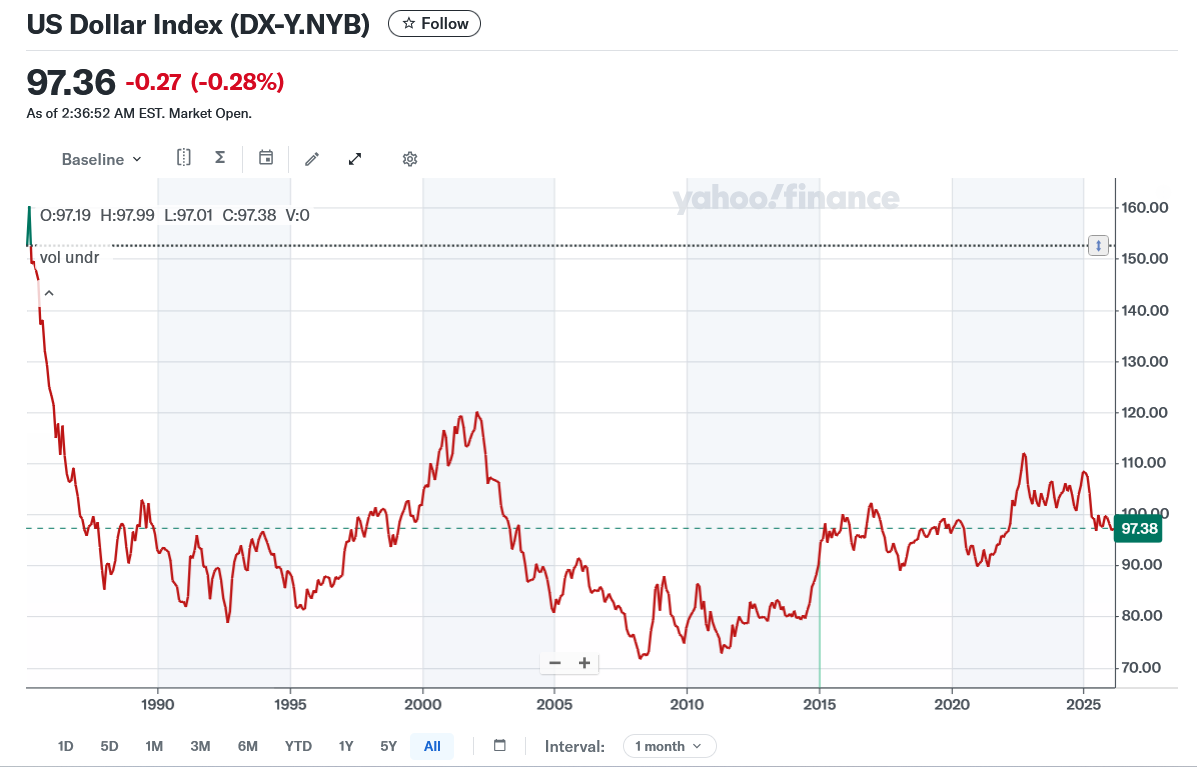
\includegraphics[height=0.46\textheight,keepaspectratio]{figures/slide08_img0_flat.png}
\end{figure}
\end{column}
\begin{column}{0.40\textwidth}
\small \textbf{U.S.\ Dollar Index (DXY):} the trade-weighted value of the USD against a basket of major currencies (EUR, JPY, GBP, CAD, SEK, CHF).
\begin{center}\small Source: Yahoo Finance\end{center}
\end{column}
\end{columns}
\end{frame}

% [src: 9]
\begin{frame}{The Dollar's Long Run: DXY by Decade}
\begin{table}
\centering
\footnotesize
\begin{tabular}{llll}
\toprule
\textbf{Decade} & \textbf{Approx.\ average level} & \textbf{Trend} & \textbf{Dominant regime} \\
\midrule
1980s & $\sim$125--140 & Peak \& crash & Super-strong USD $\to$ Plaza Accord \\
1990s & $\sim$95--105 & Mild uptrend & Strong-dollar era \\
2000s & $\sim$85--95 & Downtrend & Weak USD, commodity supercycle \\
2010s & $\sim$85--100 & Uptrend & Post-crisis recovery \\
2020s & $\sim$90--112 & Volatile & COVID slump $\to$ tightening surge $\to$ flat near 99 \\
\bottomrule
\end{tabular}
\end{table}
\end{frame}

% [src: 10]
\begin{frame}{The Largest of All Financial Markets}
FX markets facilitate international trade, raising capital abroad, transfer of risk, and speculation.
\begin{itemize}
  \item Global FX turnover averaged \textbf{\$9.6 trillion per day} (BIS Triennial Survey, April 2025)
  \item Versus roughly \$80--300 billion per day on the NYSE
\end{itemize}
\begin{columns}
\begin{column}{0.52\textwidth}
\begin{figure}
\centering
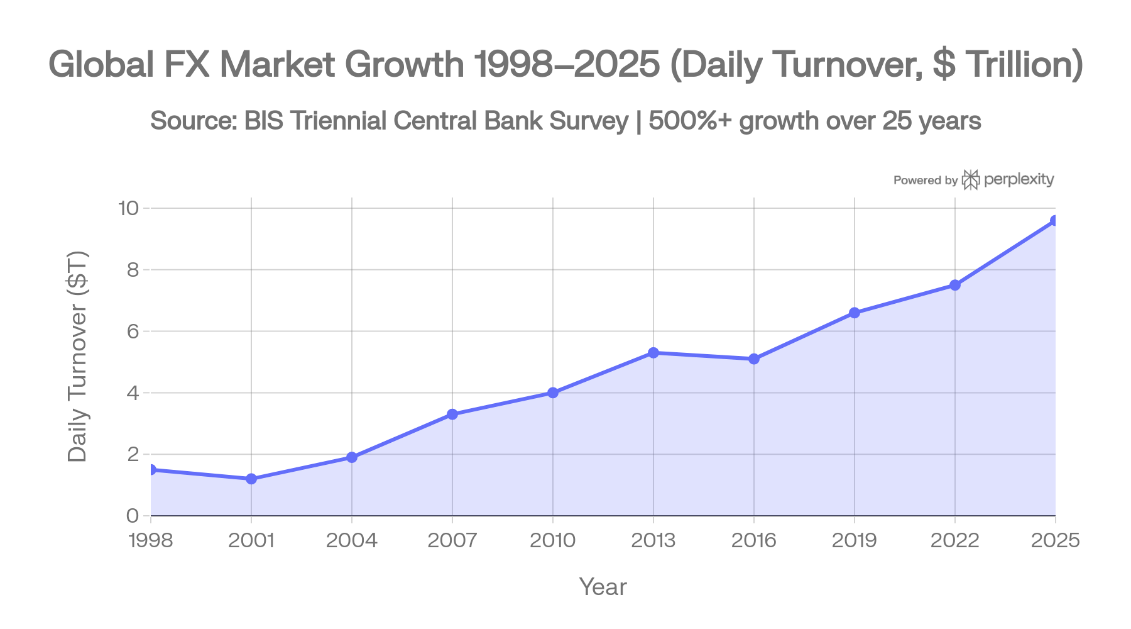
\includegraphics[width=\linewidth,keepaspectratio]{figures/slide10_img0_flat.png}
\end{figure}
\end{column}
\begin{column}{0.44\textwidth}
\begin{figure}
\centering
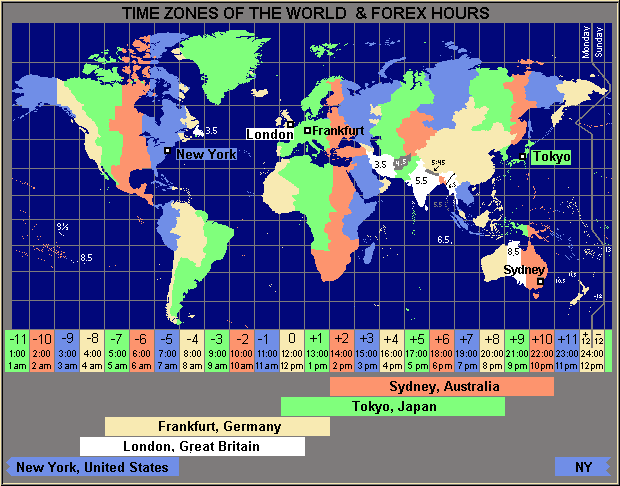
\includegraphics[height=0.44\textheight,keepaspectratio]{figures/slide11_img0.png}
\end{figure}
\end{column}
\end{columns}
\note{This is the world's largest market!}
\end{frame}

% [src: 11]
% (24-hour trading figure shown on previous frame)

% [src: 12]
\begin{frame}{Stylized Facts}
\begin{itemize}
  \item Most traded currencies: \textbf{USD, EUR, JPY, GBP}; most traded pairs: USD per EUR, JPY per USD, USD per GBP, USD per AUD
  \item Counterparties: mostly \emph{financial institutions} trading, not companies
  \item Types of transactions: spots (transact now, deliver now); forwards (transact now, deliver later); FX swaps (paired transactions, e.g., spot + forward)
  \item Horizons: forwards and swaps are mainly short-dated ($\sim$7 days) --- mainly short-term speculation
\end{itemize}
\vspace{0.3em}
\begin{center}\small Source: BIS Triennial Central Bank Survey (latest: April 2025; next: April 2028)\end{center}
\note{An FX swap is a contract in which one party borrows one currency from, and simultaneously lends another to, the second party. Each party uses the repayment obligation as collateral, with the repayment amount fixed at the FX forward rate at the start of the contract. Each day the FX market opens in Australia/New Zealand, then Asia, Europe, and North America.}
\end{frame}

% [src: 13, 14]
\begin{frame}{Where FX Trades, and What Trades Most}
\begin{columns}
\begin{column}{0.48\textwidth}
\begin{figure}
\centering
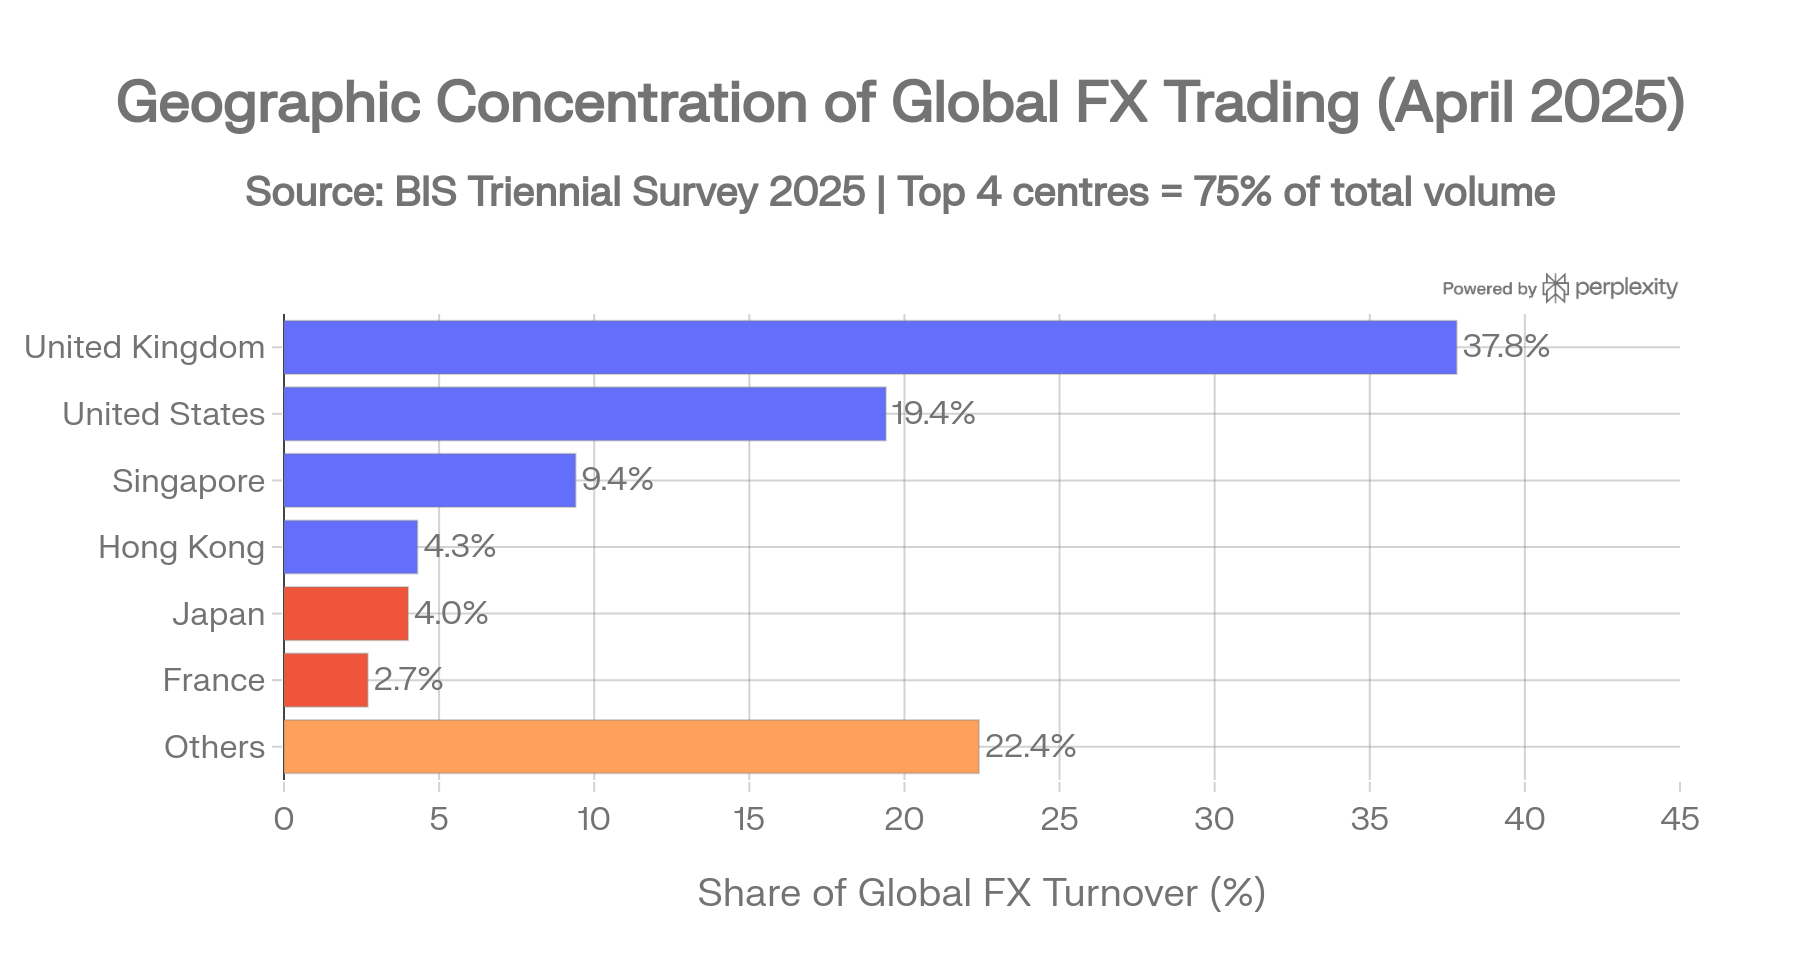
\includegraphics[width=\linewidth,keepaspectratio]{figures/slide13_img0_flat.png}
\end{figure}
\end{column}
\begin{column}{0.48\textwidth}
\begin{figure}
\centering
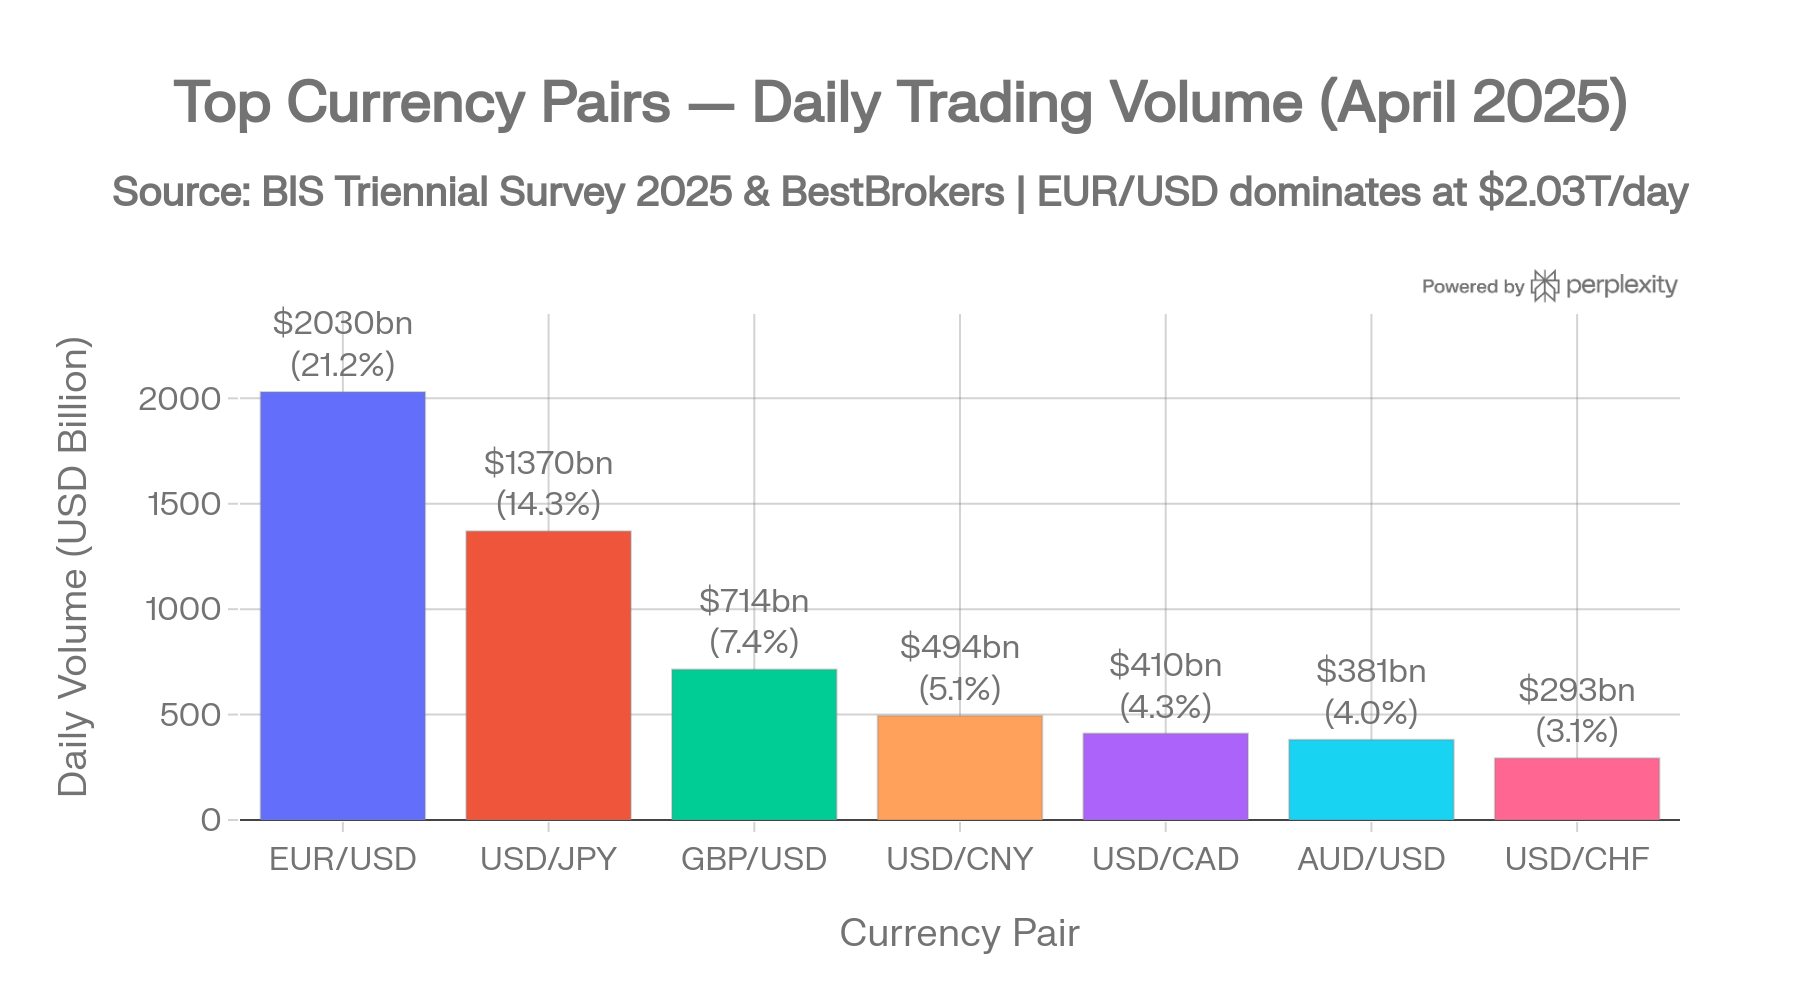
\includegraphics[width=\linewidth,keepaspectratio]{figures/slide14_img0_flat.png}
\end{figure}
\end{column}
\end{columns}
\begin{center}\small Top FX trading centers and top currency pairs --- Source: BIS Triennial Central Bank Survey (April 2025; next 2028)\end{center}
\note{FX dealer life in Singapore is hard because of long hours.}
\end{frame}

% [src: 15, 16]
\begin{frame}{Reserves and Instruments}
\begin{columns}
\begin{column}{0.48\textwidth}
\begin{figure}
\centering

\includegraphics[width=\linewidth,keepaspectratio]{figures/slide15_img0_flat.png}
\end{figure}
\end{column}
\begin{column}{0.48\textwidth}
\begin{figure}
\centering
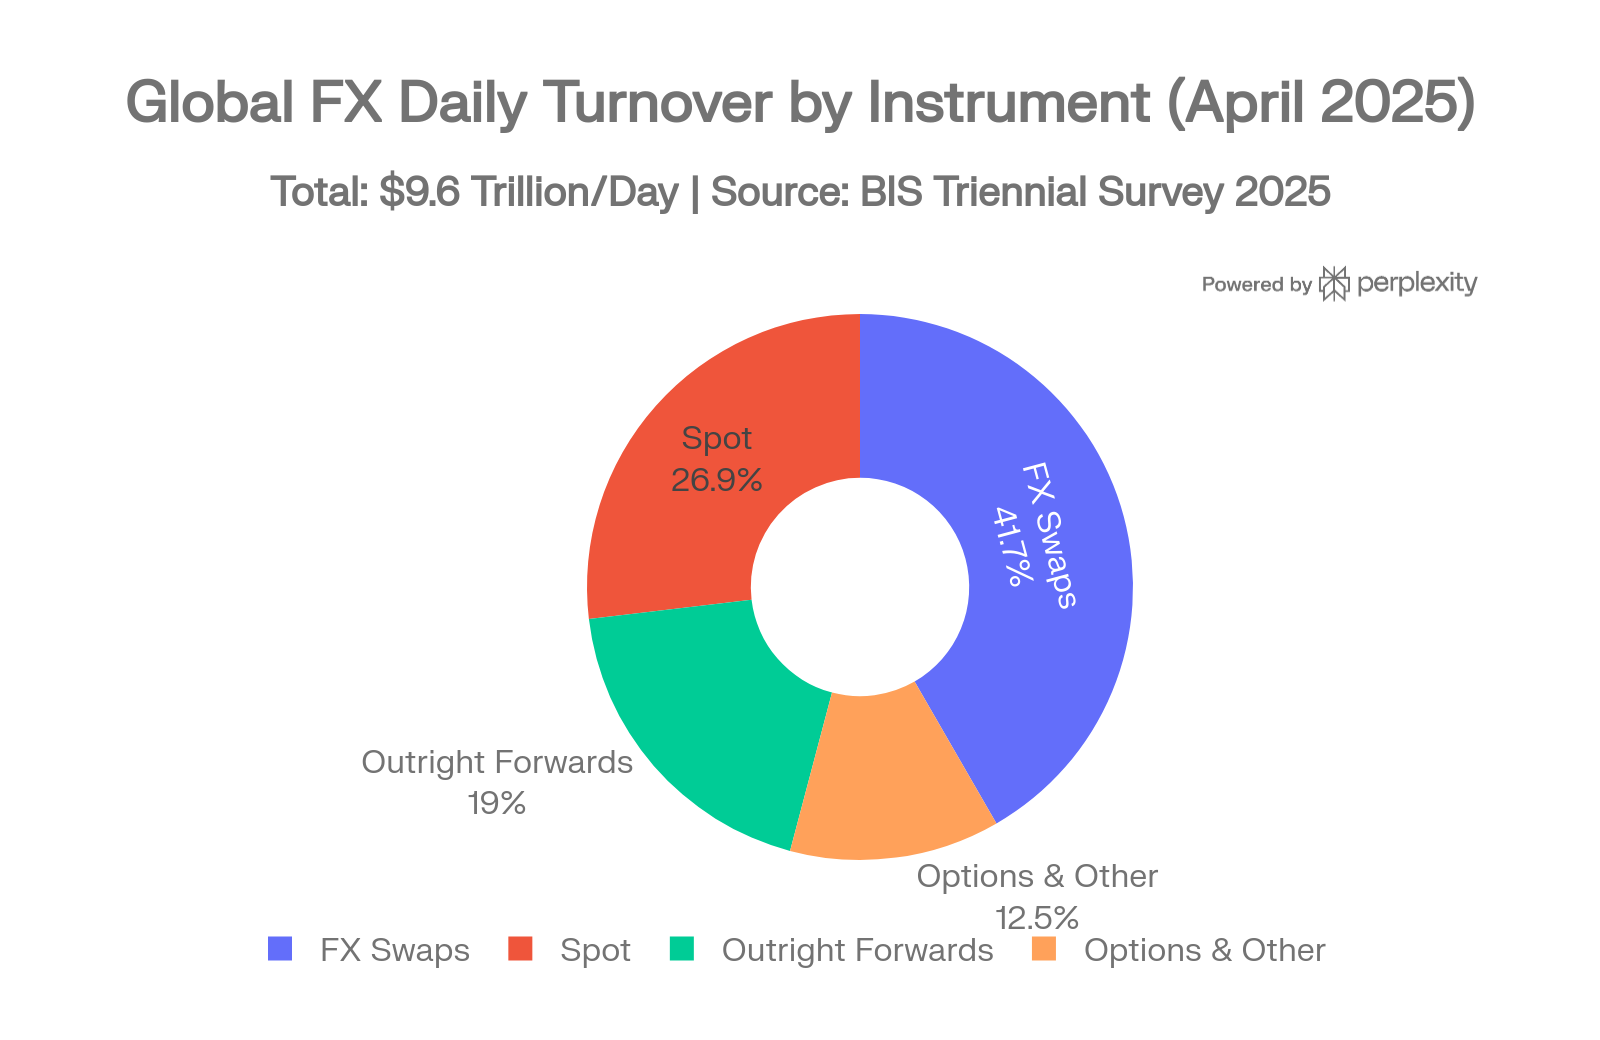
\includegraphics[width=\linewidth,keepaspectratio]{figures/slide16_img0_flat.png}
\end{figure}
\end{column}
\end{columns}
\begin{center}\small USD \& EUR share of global FX reserves; FX turnover by instrument --- Source: BIS Triennial Central Bank Survey (April 2025)\end{center}
\note{FX swaps: transactions involving the actual exchange of two currencies (principal only) on a specific date at a rate agreed at the contract, and a reverse exchange at a future date at a rate agreed at the contract. Currency swaps: contracts committing two counterparties to exchange streams of interest payments in different currencies.}
\end{frame}

% [src: 17, 18]
\begin{frame}{Dollar Dominance --- and Renminbi Internationalization}
\begin{itemize}
  \item The USD is involved in $\sim$\textbf{88\%} of all FX transactions (one side) --- unchanged for over two decades; deep network effects (Thailand buying Brazilian cotton typically goes through USD)
  \item But the dollar's share of allocated reserves has fallen from over 70\% in 2000 to roughly \textbf{57\%}, its lowest since the mid-1990s (IMF COFER, Q1 2026): euro $\sim$20\%, yen $\sim$5\%, pound $\sim$5\%, RMB $\sim$2\%
  \item \textbf{RMB internationalization} since 2009: cross-border trade settlement, bilateral swap lines with 30+ countries, CIPS, IMF SDR inclusion (2016) --- yet still far behind USD, EUR, JPY
  \item \textbf{2025--26 tariff cycle:} US tariffs on China peaked at 145\% in April 2025, and the Supreme Court struck down the IEEPA tariffs in February 2026 --- yet the renminbi \emph{appreciated}, from 7.4 to 6.8 per dollar. Why would a currency strengthen into a trade war?
  \item The fundamental constraint is \textbf{capital controls}: without free convertibility and deep, open capital markets, the RMB cannot be a genuine reserve asset
\end{itemize}
\note{2025--26 tariff cycle, answer hints: dollar-side weakness (the dollar fell $\sim$9\% in 2025), rate differentials, PBoC fixing, China's export surplus. Timeline: tariff peak April 2025, Geneva truce May 2025, SCOTUS strikes down IEEPA tariffs February 2026; CNY went from $\sim$7.4 offshore (early 2025) to $\sim$6.8 (Feb 2026).}
\end{frame}

% ============ QUOTES ============

% [src: 19]
\section{FX Market Quotes and Trades}

% [src: 20]
\begin{frame}{Types of Quotes}
\textbf{Market convention:} all currencies quoted in \emph{foreign currency per USD} (\textbf{European terms}) --- except \textbf{EUR, GBP, AUD, NZD}, quoted in American terms.
\vspace{0.2em}
\begin{description}
  \item[Direct quote] Home currency per unit of foreign currency --- for a U.S.\ firm: 0.14 USD per CNY
  \item[Indirect quote] Foreign currency per unit of home currency --- 6.94 CNY per USD
  \item[European terms] Foreign currency per USD; \textbf{American terms}: USD per unit of foreign currency
\end{description}
\begin{columns}
\begin{column}{0.52\textwidth}
\begin{figure}
\centering

\includegraphics[height=0.32\textheight,width=\linewidth,keepaspectratio]{figures/slide20_img0.png}
\end{figure}
\end{column}
\begin{column}{0.42\textwidth}
\begin{figure}
\centering
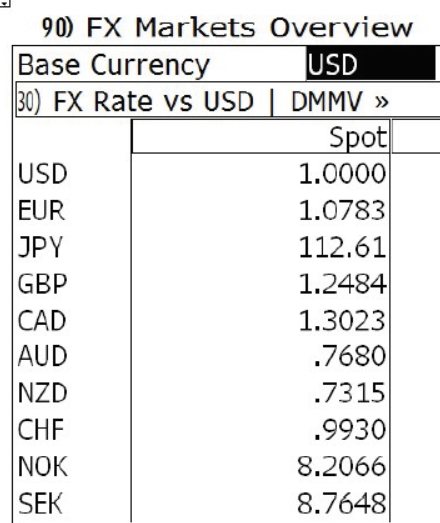
\includegraphics[height=0.32\textheight,width=\linewidth,keepaspectratio]{figures/slide20_img1.png}
\end{figure}
\end{column}
\end{columns}
\end{frame}

% [src: 21]
\begin{frame}{Cross Rates}
Exchange rates between two non-USD currencies are \textbf{cross rates}, derived from their USD quotes.
\begin{figure}
\centering

\includegraphics[height=0.58\textheight,keepaspectratio]{figures/slide21_img0_flat.png}
\end{figure}
\end{frame}

% [src: 22, 23]
\begin{frame}{Bid--Ask Spread}
Usually no explicit FX commission --- but there is a bid--ask spread (e.g., GBP per USD: 0.8395 bid / 0.8396 ask). \textbf{Bid and ask are from the dealer's perspective:}
\begin{itemize}
  \item \textbf{Bid} 0.8395: the dealer \emph{buys} USD (the reference currency) at this price --- the price you get when selling
  \item \textbf{Ask} 0.8396: the dealer \emph{sells} USD at this price --- the price you pay when buying
\end{itemize}
\begin{figure}
\centering
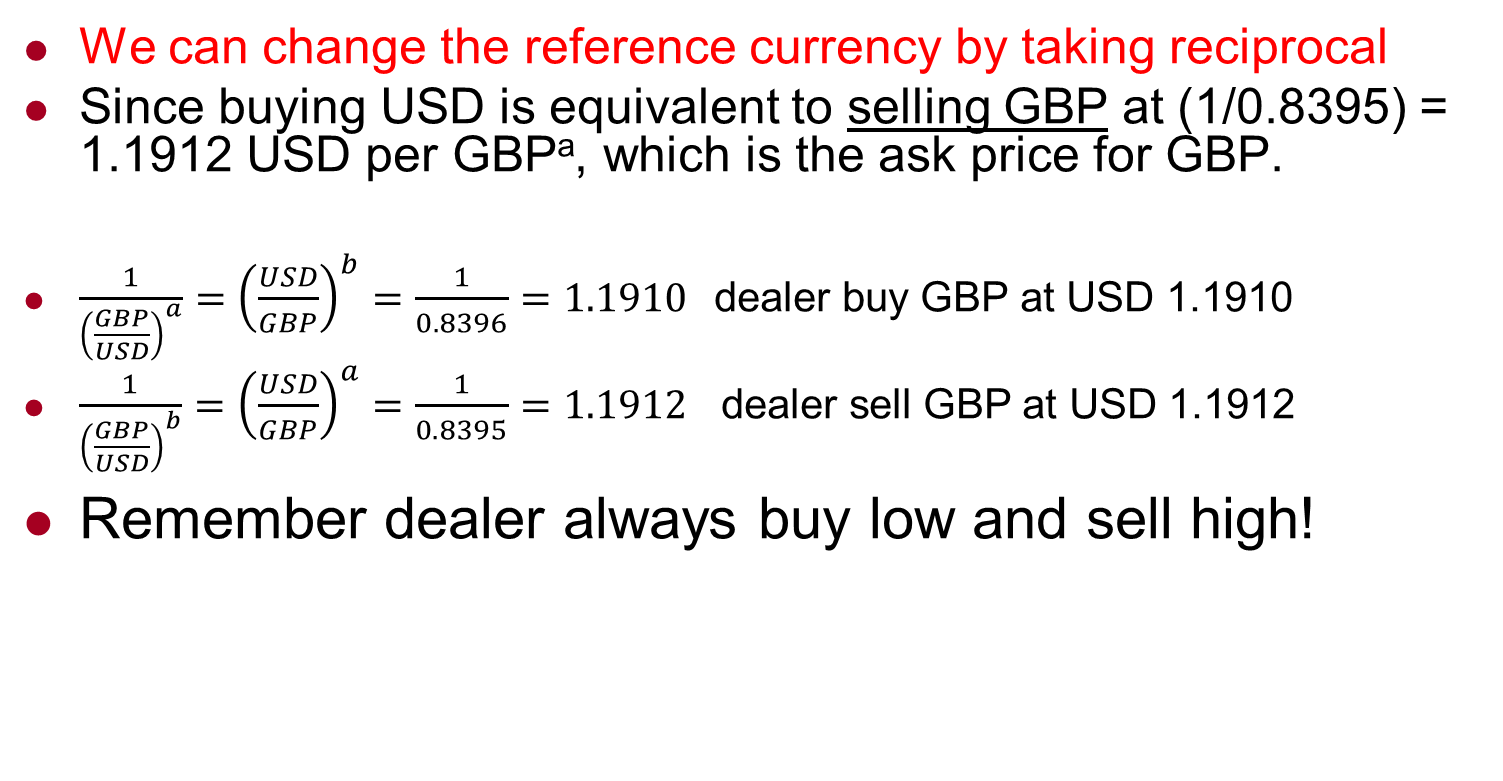
\includegraphics[height=0.44\textheight,keepaspectratio]{figures/slide23_img0_flat.png}
\end{figure}
\end{frame}

% [src: 24]
\begin{frame}{Technology and the Future of FX Markets}
Electronic trading has compressed bid--ask spreads (price efficiency), democratized access (buy-side firms stream quotes), and enabled sophisticated execution algorithms.
\begin{table}
\centering
\small
\begin{tabular}{lll}
\toprule
\textbf{Era} & \textbf{Dominant structure} & \textbf{Key innovation} \\
\midrule
Pre-1990s & Voice brokers, bilateral dealer calls & Reuters terminal \\
1990s & Electronic platforms emerge & EBS, Reuters 2000 \\
2000s & ECNs proliferate; HFT begins & FXall, 360T, co-location \\
2010s & Multi-dealer platforms dominate & Algorithmic execution suites \\
2020s & AI-integrated, real-time analytics & LLM sentiment, ML execution \\
\bottomrule
\end{tabular}
\end{table}
\end{frame}

% ============ HEDGING ============

% [src: 25]
\section{Hedging Foreign Exchange Risk}

% [src: 26, 27]
\begin{frame}{The Importance of Hedging FX Risk}
Today's companies operate globally; FX movements affect profitability and performance of domestic firms.
\vspace{0.3em}
\textbf{Boeing example:} sells planes to a Brazilian buyer for \$15 million when the dollar is worth 2 reals.
\begin{itemize}
  \item Cost to the buyer: $\$15\text{m} \times 2 = 30$ million reals
  \item If the dollar strengthens to 2.5 reals: $\$15\text{m} \times 2.5 = 37.5$ million reals --- the buyer may switch to Airbus and pay in euros
\end{itemize}
\vspace{0.3em}
\textbf{How internationally active firms hedge:} derivatives (swaps, futures); borrowing in the same currency in which they earn revenues; locating production facilities (and incurring local-currency costs) where they earn revenues.
\note{Airbus is a European consortium that makes airplanes and competes with Boeing.}
\end{frame}

% [src: 28]
\begin{frame}{Foreign Exchange Risk: FI Example}
A U.S.\ FI holds: \textbf{Assets} --- \$100m 1-yr USD loan at 9\% $+$ \pounds62.5m 1-yr UK loan at 15\%; \textbf{Liabilities} --- \$200m 1-yr USD deposits at 8\%. Spot rate: \$1.6/\pounds{} ($\pounds 62.5$m $=$ \$100m).
\begin{itemize}
  \item \textbf{If the spot rate is unchanged:} UK loan returns $\pounds62.5(1.15)\times1.6 = \$115$m ($15\%$); net return $= 0.5(9\%) + 0.5(15\%) - 8\% = \mathbf{4\%}$
  \item \textbf{If GBP depreciates to \$1.45/\pounds:} UK loan worth $\pounds62.5(1.15)\times1.45 = \$104.22$m ($4.22\%$); net return $= 0.5(9\%) + 0.5(4.22\%) - 8\% = \mathbf{-1.39\%}$
\end{itemize}
\end{frame}

% [src: 29, 30]
\begin{frame}{Hedging On the Balance Sheet}
\textbf{On-balance-sheet hedging} matches foreign assets and liabilities --- FX-driven decreases in asset values are offset by decreases in liability values (and vice versa).
\vspace{0.3em}
\textbf{Example (continued):} fund the \pounds62.5m UK loan with equivalent 1-yr pound deposits at 11\%.
\begin{itemize}
  \item No FX move: net return $= (0.5\cdot9\%+0.5\cdot15\%) - (0.5\cdot8\%+0.5\cdot11\%) = 2.5\%$
  \item GBP falls to \$1.45: UK assets yield 4.22\%; UK liability costs $\pounds62.5(1.11)\times1.45 = \$100.59$m (only 0.59\%)
  \item Net return $= (0.5\cdot9\%+0.5\cdot4.22\%) - (0.5\cdot8\%+0.5\cdot0.59\%) = 6.61\% - 4.295\% = \mathbf{2.315\%}$ --- similar to the no-movement case
\end{itemize}
\end{frame}

% [src: 31]
\begin{frame}{Hedging Off the Balance Sheet}
\textbf{Off-balance-sheet hedging} uses \emph{forward contracts}: rates locked in at $t=0$ apply at $t=1$ regardless of the prevailing spot.
\vspace{0.3em}
\textbf{Example (continued):} the FI sells the expected UK proceeds forward at \$1.55/\pounds{} for 1-yr delivery.
\begin{itemize}
  \item At year-end it delivers $\pounds62.5(1.15)$m and receives $\pounds62.5 \times 1.15 \times 1.55 = \$111.406$m --- a guaranteed 11.406\% dollar return
  \item Net return $= 0.5(9\%) + 0.5(11.406\%) - 8\% = \mathbf{2.203\%}$ --- hedged at low cost
\end{itemize}
\end{frame}

% ============ HOW DO RATES MOVE? ============

% [src: 32]
\section{How Do Exchange Rates Move?}

% [src: 33]
\begin{frame}{How Do Exchange Rates Move?}
Theories describing how exchange rates \emph{should} move:
\begin{itemize}
  \item Purchasing Power Parity (PPP) and Relative PPP
  \item Interest Rate Parity (IRP)
\end{itemize}
\vspace{0.2em}
Most parity conditions rely on the \textbf{law of one price}, which must hold in a no-arbitrage equilibrium --- arbitrage is the simultaneous buying and selling of assets for a risk-free profit.
\vspace{0.3em}

But how do rates \emph{actually} move? Does uncovered interest parity hold? If not, the \textbf{carry trade} can profit from it.
\end{frame}

% [src: 34]
\begin{frame}{Absolute Purchasing Power Parity}
The exchange rate between two currencies equals the ratio of the two countries' price levels for an identical basket of goods:
\[
S_{\text{USD/EUR}} = \frac{P_{\text{US}}}{P_{\text{Europe}}}
\]
\textbf{Example:} a basket costs \$100 in the U.S.\ and EUR 90 in Europe:
\[
S = \frac{100}{90} = 1.1111 \text{ USD per EUR}
\]
\end{frame}

% [src: 35, 36]
\begin{frame}{Big Mac Currencies: PPP in Practice}
At the end-2025 reading, a Big Mac cost \$5.99 in the U.S.\ and 7.30 francs in Switzerland (the index is updated each January and July --- treat the numbers as illustrative).
\begin{itemize}
  \item PPP-implied rate: $5.99/7.30 = 0.82$ USD per CHF; actual rate: 1.29 USD per CHF
  \item Swiss Big Mac in USD terms: \$9.42 --- too expensive by $(9.42/5.99)-1 = \mathbf{57\%}$
  \item For PPP to hold, Swiss prices in USD must fall 57\% (the CHF must depreciate)
\end{itemize}
\begin{figure}
\centering
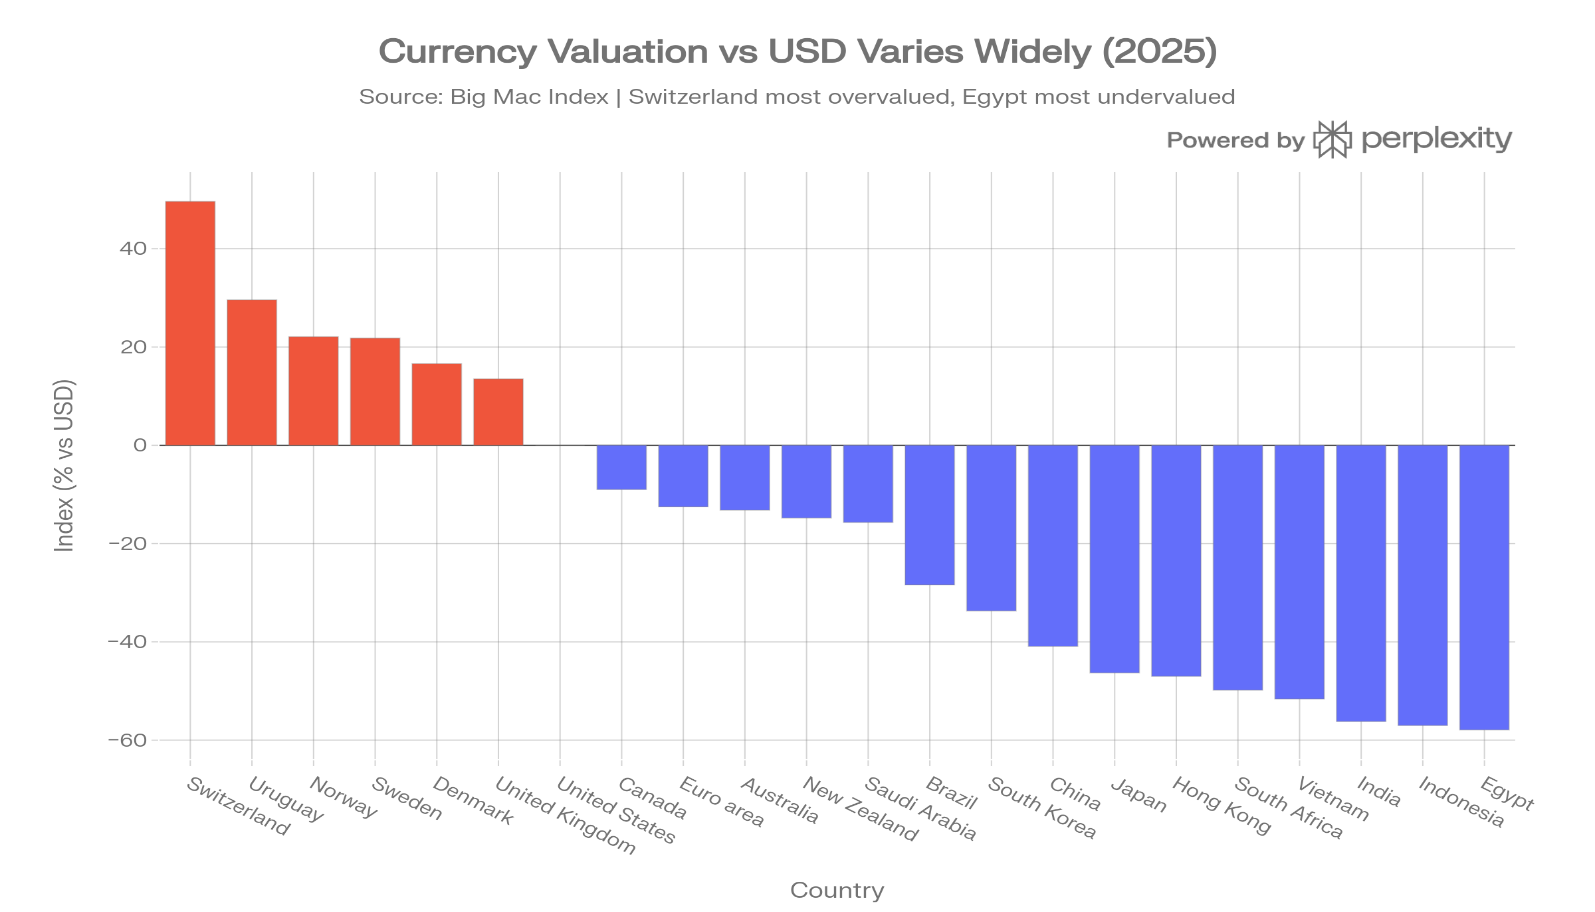
\includegraphics[height=0.42\textheight,keepaspectratio]{figures/slide36_img0_flat.png}
\end{figure}
\begin{center}\small The Big Mac index (\emph{The Economist}, since 1986), 2025: over/undervaluation vs.\ USD\end{center}
\note{\url{https://www.economist.com/content/big-mac-index}}
\end{frame}

% [src: 37]
\begin{frame}{Relative Purchasing Power Parity}
Absolute PPP rarely holds; \textbf{relative PPP} predicts the \emph{rate of change}:
\[
\%\Delta S_{\text{USD/EUR}} = \pi_{\text{US}} - \pi_{\text{EUR}}
\]
The currency of the lower-inflation country \textbf{appreciates} over time.
\vspace{0.3em}

\textbf{Example:} if U.S.\ inflation is 5\% and Euro-area inflation is 3\%, the dollar should depreciate by roughly $5\%-3\% = 2\%$ per year against the euro.
\end{frame}

% [src: 38, 39]
\begin{frame}{Interest Rate Parity (IRP) and Forward Contracts}
\begin{description}
  \item[Forward contract] Locks in a rate today to transact foreign currency in the future; settlement on a future date by maturity of the contract (commonly 1 week, 1M, 3M). \emph{Spot}: transact today, settle T+2
\end{description}
\vspace{0.2em}
IRP is an \textbf{arbitrage condition} holding when currency and money markets are in equilibrium. Two one-year strategies must yield the same (riskless) return:
\begin{enumerate}
  \item Invest \$1 in the U.S.\ at $r_{\$}$ p.a.
  \item Convert \$1 to foreign currency at $S$, invest at $r_{FC}$ p.a., and sell the proceeds \emph{forward} at $F$
\end{enumerate}
Forward contracts completely hedge the risk of future currency movements.
\note{Spot next deliver tomorrow; tomorrow next, close tomorrow.}
\end{frame}

% [src: 40, 41]
\begin{frame}{Interest Rate Parity: Derivation}
Strategy 1 (invest domestically): return $= 1 + r_D$.
\vspace{0.2em}
Strategy 2 (invest abroad, covered): convert at $S$, invest at $r_F$, convert back at the forward rate:
\[
\frac{1}{S}\times(1+r_F)\times F = \frac{F}{S}(1+r_F)
\]
Both are riskless, so they must be equal:
\[
1 + r_D = \frac{F}{S}(1+r_F)
\qquad\Longrightarrow\qquad
F = S \times \frac{1+r_D}{1+r_F}
\]
The forward rate exactly offsets the interest differential --- the currency with the higher interest rate trades at a forward \textbf{discount}.
\end{frame}

% [src: 42, 44]
\begin{frame}{Covered Interest Arbitrage (CIA)}
Compare the \textbf{domestic return} $1+r_D$ with the \textbf{foreign covered return} $\frac{F}{S}(1+r_F)$:
\begin{itemize}
  \item If $1+r_D > \frac{F}{S}(1+r_F)$: the domestic currency is overvalued in the forward market --- invest domestically
  \item If $\frac{F}{S}(1+r_F) > 1+r_D$ (e.g., a 5\% U.S.\ rate vs.\ a 7\% German rate not offset by the forward premium): borrow domestic, convert, invest foreign, sell forward --- invest in the foreign country
\end{itemize}
\vspace{0.2em}
\textbf{How CIA corrects mispricing:} arbitrage flows bid up the spot rate $S$ (or push down $F$) until
\[
\frac{F}{S}(1+r_F) = 1+r_D \qquad \text{--- IRP restored.}
\]
\end{frame}

% [src: 43]
\begin{frame}{Covered Interest Arbitrage: Example}
IRP does not hold: borrow USD at 2.405\%, convert to EUR, invest EUR at 1.36\%, sell EUR 6-month forward.
\begin{itemize}
  \item Borrow \$1m at 2.405\% (6-mo)
  \item Convert at spot \$1.1939/EUR $\to$ EUR 837{,}591.09
  \item Invest at 1.36\% $\to$ EUR 848{,}982.33 in 6 months
  \item Sell 6-month forward at \$1.2072/EUR $\to$ \$1{,}024{,}891.47
  \item Repay \$1{,}024{,}050 $\Rightarrow$ \textbf{risk-free profit \$841.47}
\end{itemize}
\begin{figure}
\centering
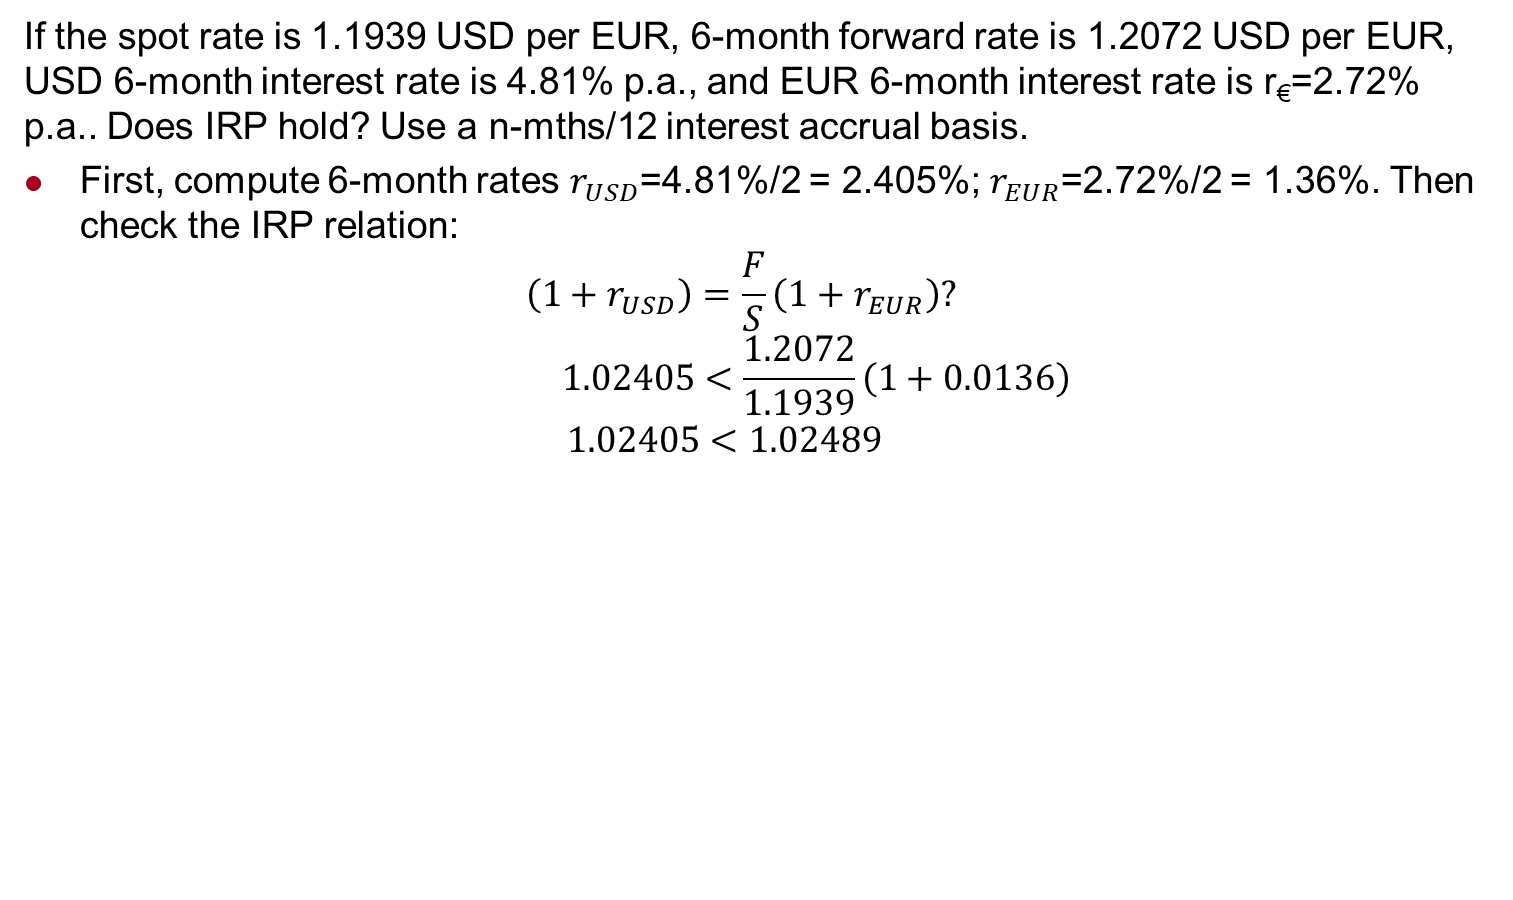
\includegraphics[height=0.34\textheight,keepaspectratio]{figures/slide43_img0_flat.png}
\end{figure}
\end{frame}

% [src: 45, 46, 47]
\begin{frame}{Three Exchange Rate Regimes}
The IMF classifies arrangements by \emph{de facto} behavior, which often differs from the announced regime.
\begin{description}
  \item[Hard pegs] No separate legal tender (dollarization: Ecuador, El Salvador; monetary union: Eurozone) or currency board --- domestic currency fully backed by reserves at a fixed rate (Hong Kong's Linked Exchange Rate System: HKD 7.80/USD since 1983). Maximum credibility, no FX risk for trade --- but loss of monetary independence and lender-of-last-resort function
  \item[Soft pegs] Conventional peg ($\pm$1\% of a central rate, e.g., Gulf states), crawling peg (adjusted at a predetermined rate to control inflation), stabilized arrangements. Some flexibility --- but vulnerable to speculative attack when fundamentals diverge
  \item[Floating] Managed float (discretionary intervention based on payments, reserves, market conditions) and freely floating (market-determined; intervention only to moderate excessive volatility)
\end{description}
\end{frame}

% [src: 48]
\begin{frame}{The Impossible Trinity (Trilemma)}
The Mundell--Fleming trilemma: a country cannot simultaneously maintain all three of \textbf{a fixed exchange rate}, \textbf{free capital mobility}, and \textbf{independent monetary policy}. Only two can coexist:
\begin{itemize}
  \item \textbf{Eurozone:} fixed rates $+$ free capital $\to$ surrendered monetary policy
  \item \textbf{Hong Kong SAR:} fixed rate $+$ free capital $\to$ no independent monetary policy; HIBOR tracks the Fed Funds Rate
  \item \textbf{China (historically):} fixed rate $+$ monetary independence $\to$ imposed capital controls
  \item \textbf{U.S./UK/Japan:} free float $+$ free capital $\to$ full monetary independence
\end{itemize}
\end{frame}

% ============ CARRY TRADE ============

% [src: 49]
\section{Carry Trade and Other Currency Strategies}

% [src: 50]
\begin{frame}{Invest in High-Interest-Rate Currencies?}
All parity conditions --- relative PPP, IRP --- predict that high-interest-rate currencies \emph{depreciate}.
\vspace{0.3em}

But most investors --- and most financial press coverage --- assume high interest rates are \emph{good} for a currency:
\begin{columns}
\begin{column}{0.32\textwidth}
\begin{figure}
\centering

\includegraphics[height=0.34\textheight,width=\linewidth,keepaspectratio]{figures/slide50_img.png}
\end{figure}
\end{column}
\begin{column}{0.32\textwidth}
\begin{figure}
\centering
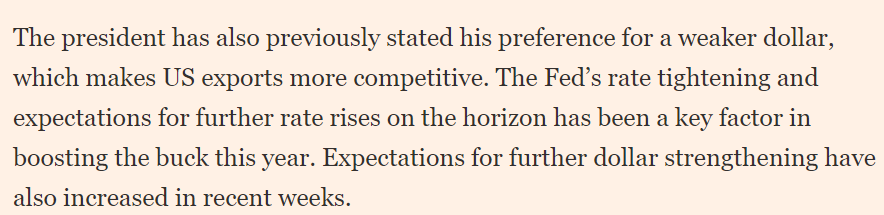
\includegraphics[height=0.34\textheight,width=\linewidth,keepaspectratio]{figures/slide50_img1.png}
\end{figure}
\end{column}
\begin{column}{0.32\textwidth}
\begin{figure}
\centering
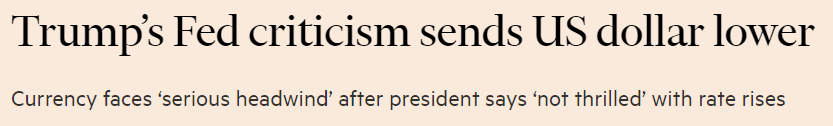
\includegraphics[height=0.34\textheight,width=\linewidth,keepaspectratio]{figures/slide50_img2.png}
\end{figure}
\end{column}
\end{columns}
\end{frame}

% [src: 51]
\begin{frame}{Uncovered Interest Rate Parity (UIRP)}
If investors are indifferent to risk, the \emph{expected} change in the spot rate offsets the interest differential --- no forward cover needed:
\[
\frac{E[S_{T}]}{S} = \frac{1+r_D}{1+r_F}
\qquad\Longleftrightarrow\qquad
E[\%\Delta S] \approx r_D - r_F
\]
High-interest-rate currencies are \emph{expected} to depreciate.
\note{Uncovered interest parity is the same as the international Fisher effect.}
\end{frame}

% [src: 52]
\begin{frame}{The Currency Carry Trade}
Hence investors like the \textbf{carry trade}: borrow low-interest currencies (e.g., JPY), invest in high-interest currencies (e.g., AUD), and \emph{do not hedge}.
\begin{itemize}
  \item If AUD depreciates (as PPP/IRP predict): you lose the additional AUD interest earned
  \item If AUD does not depreciate: you earn the interest differential
  \item Better yet, if AUD appreciates: you earn both the differential and the appreciation
\end{itemize}
\vspace{0.2em}
Many academic studies (e.g., Lustig \& Verdelhan, 2007) show the carry trade earns \textbf{positive returns} --- weird, since parity conditions say high-rate currencies should depreciate.
\end{frame}

% [src: 53]
\begin{frame}{Average Returns from Carry Trade}
\begin{figure}
\centering
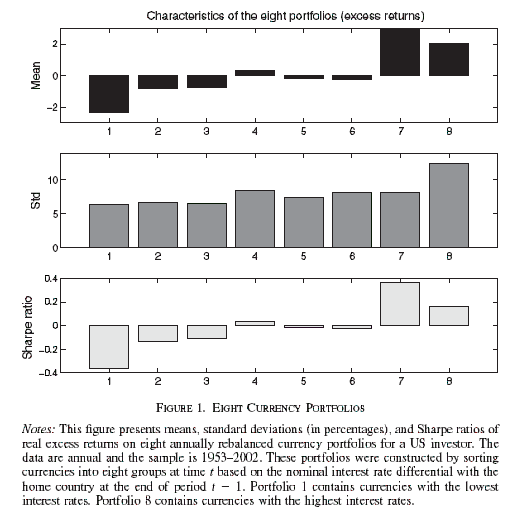
\includegraphics[height=0.64\textheight,keepaspectratio]{figures/slide53_img_conv.png}
\end{figure}
\begin{center}\small Source: Lustig \& Verdelhan (\emph{AER} 2007)\end{center}
\end{frame}

% [src: 54]
\begin{frame}{Why Does the Carry Trade Work?}
No one has a complete explanation, but suggested reasons:
\begin{description}
  \item[Equity risk] Carry-portfolio risk is related to equity risk: Lustig, Roussanov \& Verdelhan (2012) show high-interest currencies' returns are positively correlated with equity returns
  \item[Crash risk] Carry earns small positive returns most of the time but occasionally suffers large, sudden drawdowns. Carry tends to lose in ``risk-off'' episodes when volatility (VIX) spikes --- investors reduce leverage and unwind positions at the same time
\end{description}
\end{frame}

% [src: 55, 56]
\begin{frame}{Carry Trade in Bad Times}
\begin{columns}
\begin{column}{0.50\textwidth}
\begin{figure}
\centering

\includegraphics[height=0.50\textheight,keepaspectratio]{figures/slide55_img_flat.png}
\end{figure}
\begin{center}\small Yen-funded FX carry trade, 2006--2026\end{center}
\end{column}
\begin{column}{0.46\textwidth}
\begin{figure}
\centering

\includegraphics[height=0.50\textheight,keepaspectratio]{figures/slide56_img.png}
\end{figure}
\begin{center}\small HML = cumulative carry return; MSCI = U.S.\ stocks\end{center}
\end{column}
\end{columns}
\begin{center}\small From Lustig, Roussanov \& Verdelhan (2012)\end{center}
\end{frame}

% [src: 57]
\begin{frame}{Safe-Haven Currencies and Global Risk Sentiment}
A \textbf{safe-haven currency} appreciates (or holds value) during periods of heightened global risk aversion.
\begin{description}
  \item[USD] Primary safe haven: flight to dollar liquidity; reserve status creates structural dollar demand in stress
  \item[JPY] Appreciates in risk-off as carry trades unwind and Japanese investors repatriate
  \item[CHF] Current-account surplus, political neutrality, liquid capital markets
\end{description}
\vspace{0.2em}
\textbf{Risk-on} (VIX $< 15$): investors sell JPY/CHF, buy higher-yielding commodity currencies (AUD, NZD, CAD) and EM currencies; carry performs well.\\
\textbf{Risk-off} (VIX $> 25$--30): rapid flows into USD and JPY; carry unwinds; large negative tail returns.
\end{frame}

% [src: 58]
\begin{frame}{Other Currency Strategies}
\begin{description}
  \item[Currency momentum] Buy past winners, sell past losers --- a large, significant cross-sectional spread of up to 10\% p.a.\ between winner and loser portfolios (1976--2010, 40+ currencies); not highly correlated with carry --- diversification
  \item[Currency value] Buy undervalued currencies (trading below PPP), sell overvalued ones. Returns lower and more variable than carry, but value diversifies against carry crash risk
\end{description}
\vspace{0.2em}
\textbf{Combining carry, value, and momentum generates substantially higher Sharpe ratios than any single strategy alone.}
\end{frame}

% [src: 59]
\begin{frame}{Cumulative Returns of Currency Investment Strategies}
\begin{columns}
\begin{column}{0.50\textwidth}
\begin{figure}
\centering

\includegraphics[width=\linewidth,keepaspectratio]{figures/slide59_img_flat.png}
\end{figure}
\end{column}
\begin{column}{0.48\textwidth}
\begin{figure}
\centering
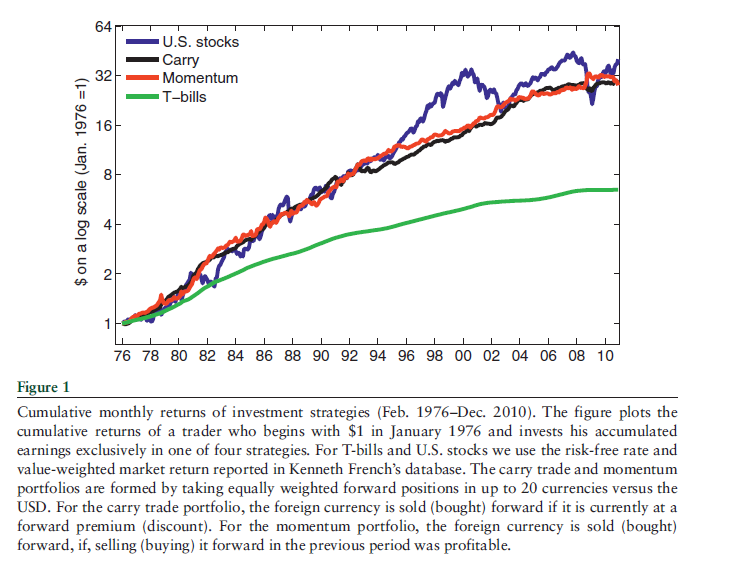
\includegraphics[width=\linewidth,keepaspectratio]{figures/slide59_img1_flat.png}
\end{figure}
\end{column}
\end{columns}
\end{frame}

% ============ SUMMARY ============

% [src: 60, 61]
\begin{frame}{Key Takeaways}
\begin{description}
  \item[FX market] Largest financial market (\$9.6T daily): currency conversion, exchange-rate setting, hedging tools; OTC, 24-hour global trading
  \item[Key terminology] Spot (immediate exchange); forward (future exchange at a pre-specified rate); cross rates (between non-USD currencies); bid--ask spread (dealer buys at bid, sells at ask)
  \item[FX risk] Currency fluctuations affect firm value; hedge on the balance sheet (match foreign assets and liabilities) or off it (forwards to lock in future rates)
  \item[PPP] Exchange rates adjust to equalize prices of identical goods across countries (Big Mac index)
  \item[IRP] Forward rates must offset interest differentials --- otherwise covered interest arbitrage
  \item[Carry trade anomaly] Borrow low-rate (JPY), invest high-rate (AUD), unhedged: violates UIRP; positive average returns but crash risk (large losses in risk-off episodes / VIX spikes)
\end{description}
\end{frame}

\end{document}
